% mechasmith: ICML 2027 submission draft.
%
% ICML 2027's author kit is not published yet. The ICML 2026 style files are vendored here as a
% stand-in. When the 2027 kit is out: drop icml2027.sty/.bst into this folder and change the two
% lines marked STYLE below. Nothing else should need to change.
\documentclass{article}

\usepackage{microtype}
\usepackage{graphicx}
\usepackage{subcaption}
\usepackage{booktabs}
\usepackage{hyperref}

\newcommand{\theHalgorithm}{\arabic{algorithm}}

\usepackage{icml2026} % STYLE: icml2027 (add [accepted] for the camera-ready)

\usepackage{amsmath}
\usepackage{amssymb}
\usepackage{mathtools}
\usepackage{amsthm}
\usepackage[capitalize,noabbrev]{cleveref}
\usepackage{xspace}
\usepackage[textsize=tiny]{todonotes}

\graphicspath{{figures/}}

\newcommand{\ms}{\textsc{mechasmith}\xspace}
\newcommand{\code}[1]{\texttt{#1}}
% Draft markers. \planned marks a claim whose experiment has not been run yet; none may remain at
% submission (grep for them).
\newcommand{\planned}[1]{\todo[inline,color=orange!25,caption={planned}]{PLANNED: #1}}
\newcommand{\note}[1]{\todo[color=blue!15,caption={note}]{#1}}

\icmltitlerunning{Robots as Code for Coding Agents}

\begin{document}

\twocolumn[
  \icmltitle{Connect, Don't Place: A Verifiable Robot Description Language\\
    for Coding Agents}

  \begin{icmlauthorlist}
    \icmlauthor{Anonymous Author(s)}{anon}
  \end{icmlauthorlist}
  \icmlaffiliation{anon}{Anonymous Institution}
  \icmlcorrespondingauthor{Anonymous Author(s)}{anon@example.com}

  \icmlkeywords{LLM agents, robot design, program synthesis, simulation, MuJoCo, embodied AI}

  \vskip 0.3in
]

\printAffiliationsAndNotice{}

\begin{abstract}
Coding agents can now write and debug substantial software, yet asking one to design a robot that
can be simulated mostly yields models that fail silently: parts float millimetres from where they
should attach, joint axes point the wrong way, links interpenetrate, and the masses are guesses.
These errors are invisible in the text of an MJCF or URDF file and surface only as odd behaviour
in simulation, long after they were made. We argue that the description language, not the agent,
is the bottleneck. We present \ms, a Python library in which a robot is one program and a part
can enter the robot only through a \emph{connection} to a part already in it; the library derives
every pose, joint anchor, axis and body frame from those connections and rejects a design with a
floating part at the line that caused it. Each build returns a machine-readable report of
verifiable properties: mass from the CAD solids, collisions at rest, the usable range of every
joint and what blocks it, and a physical test matched to the robot (standing on its actuators,
hovering, holding a payload). With this interface, six robots spanning an arm, a closed-loop
gripper, a quadrotor, a biped, a quadruped and a 29-DoF humanoid were rebuilt from public
references in 62--242 lines each, with every joint axis within 0.8\,mm of the reference's and
total mass within 6.2\% where the reference's mass is independent, and the resulting models train
locomotion policies directly.
\planned{one sentence with the headline number of the agent study (\cref{sec:agents}):
success rate of agents using \ms against agents writing MJCF/URDF or free-placement code CAD.}
\end{abstract}

\section{Introduction}
\label{sec:intro}

Simulation is where most robot learning now happens, and every simulated robot starts as a model
file: an MJCF for MuJoCo~\citep{todorov2012mujoco}, a URDF for ROS-based
stacks~\citep{quigley2009ros}, or a USD for Isaac~\citep{makoviychuk2021isaac}. Writing one is
slow, expert work, and curated collections such as MuJoCo Menagerie~\citep{zakka2022menagerie}
exist because good models are scarce. Large language models have been proposed as robot
designers~\citep{stella2023llmdesign} and used to evolve
morphologies~\citep{ringel2024text2robot,qiu2024robomorph}, but these systems search over
restricted, hand-built parameterisations. Asking a general coding agent to write a new model from
scratch exposes the problem directly: the formats encode every body as a pose relative to its
parent, so a single wrong offset produces a part that floats, a joint that turns about the wrong
axis, or two links that overlap at rest. Nothing in the file reports the error. The agent, which
is otherwise good at fixing what a tool tells it is wrong~\citep{shinn2023reflexion,madaan2023selfrefine,jimenez2024swebench},
has nothing to read.

We take the view that the design interface should make such errors unrepresentable where possible
and loud where not, and should turn every remaining property that matters into a number an agent
can read. \ms implements this view as a Python library with three commitments:

\begin{enumerate}
\item \textbf{Connect, don't place.} There is no API to position a part. A part enters the robot
  only by being fastened face to face to a connector on a part already placed, attached with a
  checked contact, or made the moving side of a joint. Placement is derived, so a robot is
  connected by construction, and a shape that does not touch what it is attached to raises an
  \code{AttachmentError} naming the gap in millimetres (\cref{sec:connect}).
\item \textbf{Everything derived.} Joint anchors, axes, kinematic tree, body frames, inertias and
  actuator limits are computed from the connections, the solids and datasheet specifications; the
  designer never writes them (\cref{sec:derive}).
\item \textbf{A report, not a picture.} A build emits MJCF, URDF and a JSON report of checks: mass
  per body, collisions at home, the usable range of each joint with the first contact that ends
  it, and a test matched to the robot class. Every parameter carries a declared range, so an agent
  can explore without leaving the space the designer validated (\cref{sec:report}).
\end{enumerate}

Our contributions are:
\begin{itemize}
\item A robot description language whose core invariant (every part is reached through a checked
  connection) removes the dominant class of silent errors in hand-written simulation models.
\item A verifier suite that converts physical validity into structured feedback suited to
  agentic iteration, from geometric checks to closed-loop simulation tests.
\item Evidence of expressiveness: six real robots rebuilt from public references, including
  closed kinematic loops, thrust-vectoring rotors and torque-controlled legged platforms, each
  matching its reference's joint axes, and models that train walking policies without further
  editing (\cref{sec:fidelity,sec:rl}).
\item \planned{A controlled study of coding agents building robots with \ms against MJCF/URDF
  authoring and free-placement code CAD, with ablations of each verifier (\cref{sec:agents}).}
\end{itemize}

\section{Related Work}
\label{sec:related}

\paragraph{Robot description formats.}
URDF~\citep{quigley2009ros} and MJCF~\citep{todorov2012mujoco} describe a robot as a tree of bodies
with explicit relative poses. Curated model collections~\citep{zakka2022menagerie} show how much
expert effort a faithful model takes. Neither format can express that two parts touch, so
connectivity is a convention rather than a checked property. \ms targets the same formats as
outputs and moves the authoring one level up.

\paragraph{Code CAD.}
Programmatic CAD kernels such as CadQuery and build123d~\citep{cadquery,build123d} make geometry
scriptable, and recent work generates CAD programs from text~\citep{khan2024text2cad}. These tools
position parts with coordinates and know nothing about joints, actuators or simulation. \ms uses
build123d as its geometry kernel but removes free placement from the interface and adds the
kinematic and physical layer.

\paragraph{Computational and evolutionary robot design.}
Co-design of morphology and control has a long history~\citep{sims1994evolving} and benchmarks
such as Evolution Gym~\citep{bhatia2021evogym}. LLM-driven variants propose designs from
text~\citep{ringel2024text2robot,qiu2024robomorph,stella2023llmdesign}. These methods search a
fixed design grammar; \ms is an open-ended language whose validity is enforced by construction and
by checks, and is complementary: it can serve as the grammar.

\paragraph{LLMs writing code against verifiers.}
Agents improve markedly when an environment returns precise feedback: on software
issues~\citep{jimenez2024swebench}, by self-reflection~\citep{shinn2023reflexion,madaan2023selfrefine},
in program search with an evaluator~\citep{romeraparedes2024funsearch}, and when writing reward
functions checked in simulation~\citep{ma2024eureka}. Generative simulation pipelines create
tasks and scenes for robot learning~\citep{wang2024robogen}. We supply the missing verifier for
the robot itself.

\paragraph{Simulation for learning.}
GPU simulators~\citep{freeman2021brax,makoviychuk2021isaac} make policy training cheap, which moves
the bottleneck to producing correct models. \ms emits primitive-collision models for MJX alongside
the mesh model (\cref{sec:rl}).

\section{\ms}
\label{sec:method}

A design is one Python file exposing a \code{build(p)} function decorated with \code{@design},
which declares typed parameters with ranges and named poses. It returns a \code{Robot}. All units
are millimetres and radians in one world frame at the home pose (x forward, y left, z up).
\Cref{fig:gallery} shows the bundled designs.

\begin{figure*}[t]
  \centering
  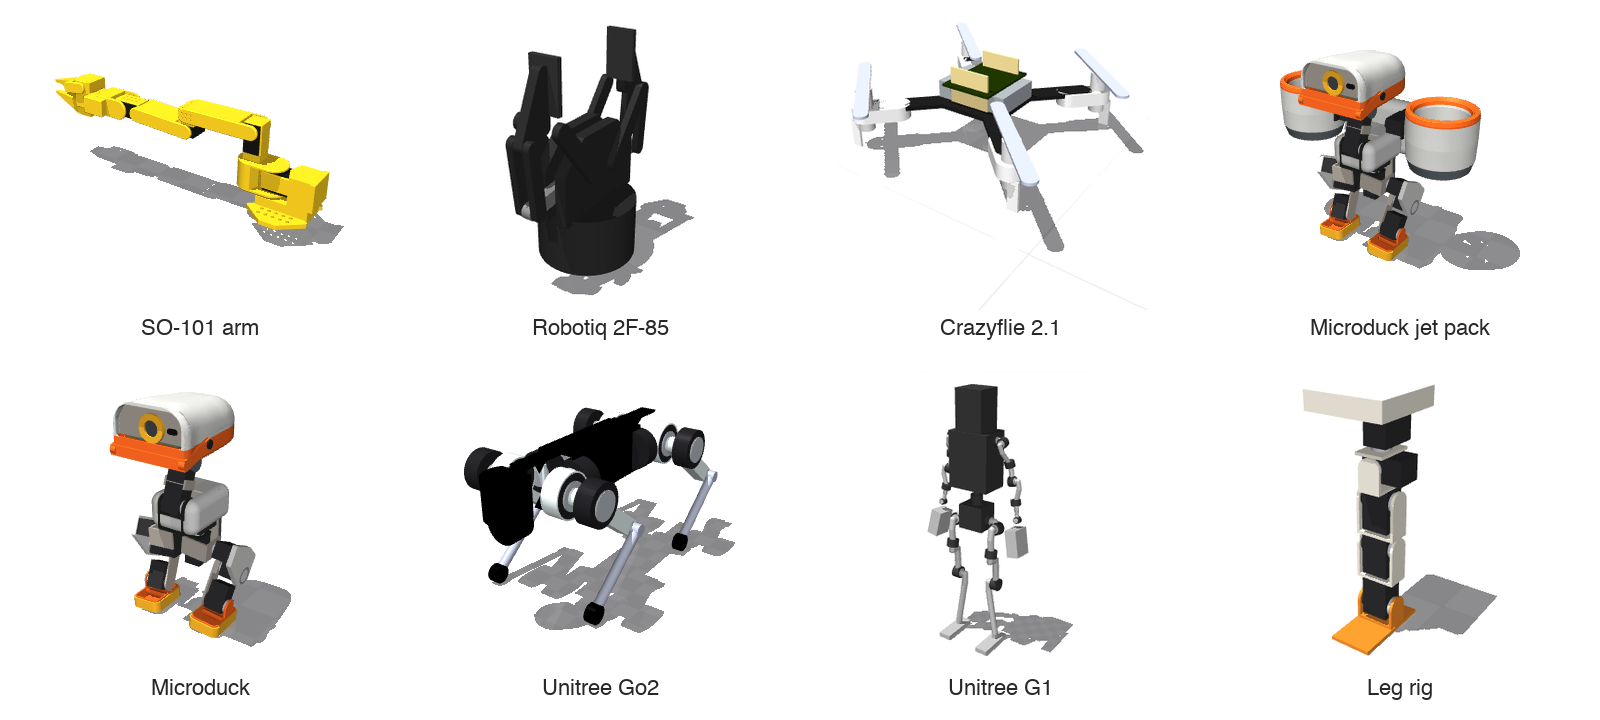
\includegraphics[width=\textwidth]{gallery.png}
  \caption{The bundled designs as built by \ms. Six are rebuilt from public reference models,
  without using the references' meshes; the jet-pack Microduck and the single leg are new designs.}
  \label{fig:gallery}
\end{figure*}

\subsection{Connections}
\label{sec:connect}
A \emph{connector} is a frame on a part's surface whose $z$ axis is the outward normal and $x$ the
reference direction. Its position is checked to lie on the part's surface when it is declared.
Parts are placed only by connection, root outward:
\begin{itemize}
\item \code{fasten(a, b, spin, at)} places $b$ so that its connector faces $a$'s, with
  normals opposed; \code{spin} fixes the free rotation about the normal and \code{at} slides
  the contact along $a$'s face (checked to stay on it).
\item \code{attach(base, part)} admits a shape drawn in world coordinates (a shell, a cover) only
  if it touches \code{base}; otherwise it raises an error reporting the gap.
\item \code{joint(name, actuator, range)} makes a placed servo or motor the joint between its
  case and its output; \code{hinge} adds an unactuated pin whose axis must pass through both
  parts, and a hinge between parts already connected closes a kinematic loop.
\item Higher-level constructors are built from these: \code{link} draws a printed link around a
  servo, cut clear of its swept volume and pocketed for the next one; \code{chain} builds a limb
  from a joint table; \code{rotor} adds thrust and reaction torque.
\end{itemize}
Because placement is computed and contact is checked at each call, the robot is a connected graph
of touching parts by construction. Re-connecting an already placed part must agree with its pose,
which catches over-constrained mistakes.
\note{Add a formal statement: invariant (every part reachable from the root through checked
contacts) and the proof sketch by induction over calls.}

\subsection{Derivation}
\label{sec:derive}
\code{robot()} contracts rigidly connected parts into links and splits them at joints, giving the
kinematic tree. Joint anchors and axes come from the actuator frames; inertias from the solids at a
material density and, for printed parts, an infill model fitted to measured masses; actuator gains,
armature and limits from datasheets (armature $=$ rotor inertia $\times$ (gear ratio)$^2$).
\code{mirror} with prefixes \code{left\_} and \code{right\_} produces the other side under an explicit axis convention,
since vendors differ in whether mirrored joints keep or flip their axes.

\subsection{The build report}
\label{sec:report}
A build writes MJCF, URDF, an MJX variant with primitive collisions, renders and a JSON report:
\begin{itemize}
\item \textbf{Mass} per body and total.
\item \textbf{Interference}: overlapping part pairs at home, and for every joint a sweep over its
  declared range reporting the usable interval and the first colliding pair at each end.
\item \textbf{Class test}: floating-base robots must hold \code{home} for 3\,s on actuator PD alone
  (reporting settled pitch, the weakest actuator and a stiffness ratio); rotorcraft are trimmed,
  disturbed by $10^\circ$ and must recover in closed loop; fixed-base arms report actuator load at
  full reach with a payload.
\end{itemize}
Every parameter override is validated against its declared range before building.
\note{Figure 2: one design snippet, the AttachmentError it raises when a number is wrong, and the
report fragment after the fix. Source: README example.}

\section{Experiments}
\label{sec:experiments}

We ask three questions. \textbf{Q1}: can the language express real robots faithfully
(\cref{sec:fidelity})? \textbf{Q2}: do coding agents build valid robots more often with it than
with existing interfaces, and which parts of it matter (\cref{sec:agents})? \textbf{Q3}: are the
models usable for learning without editing (\cref{sec:rl})?

\subsection{Q1: Rebuilding real robots}
\label{sec:fidelity}
Each of the six reference designs was built by matching a public reference model through rounds of
implement, critique, improve and rebuild; when a robot needed something the API could not express
(closed loops for the gripper, thrust for the quadrotor, torque motors for the quadruped), the
library was extended rather than the design worked around. \Cref{tab:designs} is generated from
the build reports.

\begin{table*}[t]
  \centering
  \caption{The bundled designs, from their build reports. LoC: non-blank, non-comment lines of the
  design file. $\Delta m$: total mass against the reference model (omitted where there is no
  independent reference; the G1's link masses are taken from its reference as budgets). Coll.:
  overlapping part pairs at home. Full range: joints whose sweep reaches both declared limits;
  the limits found are physical self-contacts (gripper pads meeting at closure, left and right
  feet meeting at full abduction, the SO-101 elbow stopping at 2.36\,rad as the reference's
  does). Test: the class test of \cref{sec:report}; Microduck's reference model also fails the
  actuator-only stand test at its real mass.}
  \label{tab:designs}
  % Generated by paper/scripts/collect_results.py. Do not edit by hand.
\begin{tabular}{llrrrcrl}
\toprule
Design & Type & LoC & Mass & $\Delta m$ & Coll. & Full range & Test \\
\midrule
\texttt{so101} & arm & 112 & 599.6\,g & -5.1\% & 0 & 5/6 & arm: pass \\
\texttt{robotiq\_2f85} & gripper & 62 & 1055.6\,g & +0.2\% & 0 & 0/1 & -- \\
\texttt{crazyflie2} & quadrotor & 63 & 27.1\,g & +0.4\% & 0 & -- & hover: pass \\
\texttt{microduck} & biped & 242 & 691.6\,g & -6.2\% & 0 & 8/14 & stand: fail \\
\texttt{microduck\_jetpack} & biped + fans & 141 & 1247.6\,g & -- & 0 & 8/16 & hover: pass \\
\texttt{go2} & quadruped & 125 & 14.85\,kg & -2.4\% & 0 & 6/12 & stand: pass \\
\texttt{g1} & humanoid & 69 & 33.34\,kg & -- & 0 & 15/29 & stand: pass \\
\texttt{duck\_leg} & leg & 58 & 139.3\,g & -- & 0 & 5/5 & -- \\
\bottomrule
\end{tabular}

\end{table*}

\planned{Joint-axis agreement per design from \code{scripts/compare\_joints.py} against each
reference (max distance between axis lines in mm, max angle in degrees) as two extra columns;
README reports $\le$0.2\,mm for SO-101, $\le$0.8\,mm for Microduck, coincident for the others.
Extend \code{collect\_results.py} to run it.}
\planned{Authoring effort: lines of the reference MJCF/URDF vs.\ lines of the design file.}

\subsection{Q2: Coding agents designing robots}
\label{sec:agents}
\planned{Not run yet. Design below; see \code{paper/README.md} for the protocol.}

\paragraph{Tasks.} (i) \emph{Rebuild}: given a reference's published numbers (joint table,
masses, dimensions) but not its model file, produce a model. (ii) \emph{Specify}: given a
natural-language brief (e.g.\ a 4-DoF arm reaching 300\,mm holding 100\,g), produce a design that
passes the class test. (iii) \emph{Repair}: given a design with injected faults (shifted
connector, flipped axis, oversized parent blocking a joint), fix it.

\paragraph{Conditions.} The same agent and budget with: (A) raw MJCF/URDF authoring with MuJoCo
available; (B) build123d with free placement plus a script that exports MJCF; (C) \ms; and
ablations of (C) without the contact check, without the sweep, without the class test, and
without declared parameter ranges.

\paragraph{Metrics.} Rate of valid models (loads, connected, no home collisions), joint-axis error
to the reference, mass error, class-test pass rate, iterations and tokens to first valid model.
An independent checker computes the metrics for every condition, so (A) and (B) are scored by the
same contact and sweep code that \ms uses.

\subsection{Q3: Training on generated models}
\label{sec:rl}
The MJX export of \code{microduck} trains with Brax PPO~\citep{freeman2021brax,schulman2017ppo}
to track 0.3\,m/s velocity commands with an even gait after $3\times10^8$ environment steps
(about 25 minutes on one GPU), and a single policy for \code{microduck\_jetpack} walks, hops,
flies and lands. Both use the build outputs unedited.
\planned{Report learning curves and the hardware used; state seeds and variance.}

\section{Limitations and Discussion}
\label{sec:discussion}

\paragraph{What is not checked.} The report covers connectivity, interference along single-joint
sweeps from home, mass and a short class test. It does not check multi-joint self-collision over
the whole configuration space, structural strength, manufacturability beyond 3D-printing infill,
or cable routing. Masses depend on density and infill models fitted per robot.

\paragraph{Fidelity is measured against simulation models.} Our references are public MJCF/URDF
models, themselves approximations; agreement with them is not agreement with the hardware. Masses
for parts we do not model (fasteners, wiring) explain most of the remaining gaps (e.g.\ Microduck's
legs are 10\% light).

\paragraph{Examples and library grew together.} The library was extended while the designs were
written, each robot adding what it needed. Q1 therefore shows the
language can express these robots, not that an agent finds them unaided; that is what Q2 measures.

\paragraph{Construction guarantees have edges.} Running the independent checker
(\cref{app:checker}) on our own designs found three faults in the G1 that \ms's checks had passed:
cross-piece joints whose parts overlapped by 5--7.5\,cm$^3$ inside an over-generous pin allowance,
hands drawn 29\,mm from the wrists they belong to (shapes added to a limb's last link were never
joined to it), and three structures that were invalid solids. Each was a gap in a library routine,
not in a design, so each was fixed once in the library (cross pieces are now clevis joints, and
every limb link must be a single solid), after which all eight designs pass both checkers. The
guarantee that nothing floats holds for what the connection API places; derived geometry needs
its own checks, and an independent checker is how we found where they were missing.

\paragraph{Generality.} Designs are limited to rigid bodies with revolute joints, pins and rotors.
Prismatic joints, tendons and soft parts are future work.

\section*{Impact Statement}

This work lowers the cost of producing simulation models of robots, which can speed up research in
robot learning and make it accessible to groups without mechanical design expertise. Simulation
models that pass our checks can still differ from hardware; deploying a policy trained on them to a
physical robot needs the usual validation. We do not foresee misuse specific to this work beyond
that of robotics in general.


\bibliography{refs}
\bibliographystyle{icml2026} % STYLE: icml2027

\newpage
\appendix
\onecolumn
\section{Per-robot iteration records}
\label{app:iterations}
\planned{Condense \code{docs/iterations/\{robotiq\_2f85,crazyflie2,go2,g1\}.md}: round-1
failure table, library change it drove, round-2 result.}

\section{The independent checker}
\label{app:checker}
\planned{Describe checker.py: shapes (visual geoms as exact meshes), connection rule (touch within
0.2\,mm, or a hinge axis within 3\,mm of both parts, the rule \ms enforces for its own pins),
overlap threshold (1\,mm$^3$ by mesh boolean), joint metrics and the stand test. Report that it
passes all eight bundled designs.}

\section{Agent study protocol}
\label{app:protocol}
\planned{Prompts, tool access, budgets, fault-injection procedure, checker implementation.}

\section{Reproducibility}
All numbers in \cref{tab:designs} are produced by \code{paper/scripts/collect\_results.py
--rebuild} from the repository at the submission commit.


\end{document}
